\documentclass[14pt, a4paper]{article}
\usepackage[T2A]{fontenc}
\usepackage[utf8]{inputenc}
\usepackage[russian]{babel}
\usepackage[left=3cm, right=1.5cm, top=2cm, bottom=2cm]{geometry}
\usepackage{indentfirst}
\usepackage{microtype}
\usepackage{array}
\usepackage{xcolor}
% \usepackage{times}
\usepackage{tempora}
\usepackage{ulem}
\usepackage{setspace}
\usepackage{amsmath}
\usepackage{booktabs}
\usepackage{graphicx}
\usepackage{float}
\usepackage{listings}
\graphicspath{{reports/figures/}{figures/}}
\lstset{basicstyle=\ttfamily\small, breaklines=true, columns=fullflexible, frame=single, keepspaces=true}
\pagestyle{empty}

\makeatletter
\renewcommand\section{\@startsection {section}{1}{\parindent}%
  {-3.5ex \@plus -1ex \@minus -.2ex}%
  {0.5ex}%
  {\normalfont\Large\bfseries}}
\renewcommand\tableofcontents{%
  \begin{center}\Large\bfseries\contentsname\end{center}%
  \@starttoc{toc}%
}
\renewcommand*\l@section{\@dottedtocline{1}{0em}{1.5em}}
\makeatother

\begin{document}
\onehalfspacing

\begin{center}
    \textbf{ФЕДЕРАЛЬНОЕ ГОСУДАРСТВЕННОЕ АВТОНОМНОЕ ОБРАЗОВАТЕЛЬНОЕ} \\
    \textbf{УЧРЕЖДЕНИЕ ВЫСШЕГО ОБРАЗОВАНИЯ} \\
    \textbf{«МОСКОВСКИЙ АВИАЦИОННЫЙ ИНСТИТУТ} \\
    \textbf{(НАЦИОНАЛЬНЫЙ ИССЛЕДОВАТЕЛЬСКИЙ УНИВЕРСИТЕТ)»}
\end{center}

\begin{center}
    \bfseries Институт №8 «Компьютерные науки и \\
    \bfseries прикладная математика» \\
    \bfseries Кафедра 806 «Вычислительная математика \\
    \bfseries и программирование»
\end{center}

\vspace{3cm}

\begin{center}
    \Large\bfseries Отчет \\
    \vspace{0.5cm}
    \mdseries по лабораторной работе №1.5
\end{center}

\vfill

\noindent
\hfill
\begin{tabular}{ll}
Группа:       & М8О-307Б-21 \\
Студент:      & М. С. Ивченко \\
Преподаватель:& доц. В. В. Киндинова \\
Оценка:       & \underline{\makebox[3cm][c]{}} \\ [0.2cm]
Дата:         & \underline{\makebox[3cm][c]{}}
\end{tabular}

\vfill

\begin{center}
    Москва \\
    2026
\end{center}

\newpage

\setcounter{tocdepth}{2}
\tableofcontents
\newpage

\section*{Тема}
\addcontentsline{toc}{section}{Тема}
Цель данной лабораторной работы -- рассмотреть QR-разложение как инструмент анализа матриц и решения полной проблемы собственных значений. Работа показывает, как последовательные QR-итерации позволяют находить спектр произвольной матрицы с заданной точностью.

\section*{Задание}
\addcontentsline{toc}{section}{Задание}
Реализовать алгоритм $QR$-разложения матриц в виде программы. На его основе разработать программу, реализующую $QR$-алгоритм решения полной проблемы собственных значений произвольных матриц, задавая в качестве входных данных матрицу и точность вычислений. С использованием разработанного программного обеспечения найти собственные значения матрицы.

\section*{Теория}
\addcontentsline{toc}{section}{Теория}
QR-разложение представляет матрицу в виде
\[
    A=QR,
\]
где $Q$ -- ортогональная матрица, а $R$ -- верхнетреугольная. Ортогональность означает $Q^TQ=I$, поэтому умножение на $Q$ не ухудшает норму вектора и численно устойчиво. В реализации использовались отражения Хаусхолдера. Такое отражение зануляет поддиагональные элементы выбранного столбца одним ортогональным преобразованием:
\[
    H=I-2\frac{vv^T}{v^Tv}.
\]
Последовательное применение отражений приводит исходную матрицу к верхнетреугольной форме $R$, а произведение отражений образует матрицу $Q$.

QR-алгоритм для собственных значений строит последовательность
\[
    A_k = Q_kR_k, \qquad A_{k+1}=R_kQ_k.
\]
Матрицы $A_k$ и $A_{k+1}$ подобны, так как
\[
    A_{k+1}=Q_k^TA_kQ_k.
\]
Следовательно, все матрицы последовательности имеют одни и те же собственные значения. Для матриц с действительными собственными значениями внедиагональная нижняя часть постепенно стремится к нулю, и диагональные элементы дают приближения к собственным значениям.

Если у исходной матрицы есть комплексно-сопряженная пара собственных значений, в процессе может появиться почти изолированный блок $2\times2$. Тогда собственные значения находятся как корни характеристического уравнения этого блока:
\[
    \lambda^2-\operatorname{tr}(B)\lambda+\det(B)=0.
\]
Остановка алгоритма выполняется по норме поддиагональных элементов соответствующего столбца или блока. Чем меньше заданная точность $\varepsilon$, тем больше итераций требуется, но тем меньше ошибка в найденных собственных значениях.

\begin{lstlisting}[language=Python]
Q, R = qr_decomposition(A)
A = R.dot(Q)
if np.linalg.norm(A[i+1:, i]) <= precision_epsilon:
    current_eigenvalues.append(A[i, i])
\end{lstlisting}

\section*{Ход лабораторной работы}
\addcontentsline{toc}{section}{Ход лабораторной работы}
Для матрицы
\[
A=\begin{pmatrix}
7&6&-3\\
5&-6&8\\
-7&4&-5
\end{pmatrix}
\]
проверка QR-разложения дала $\|QR-A\|_{\max}=1.78\cdot10^{-15}$. QR-алгоритм при $\varepsilon=10^{-6}$ нашел
\[
    \lambda=(-13.98262585,\;8.90665239,\;1.07597346),
\]
что совпадает с эталонным результатом NumPy до заданной точности. Также была проверена матрица поворота, для которой алгоритм вернул комплексную пару $\pm i$ и значение $2$.

\begin{figure}[H]
    \centering
    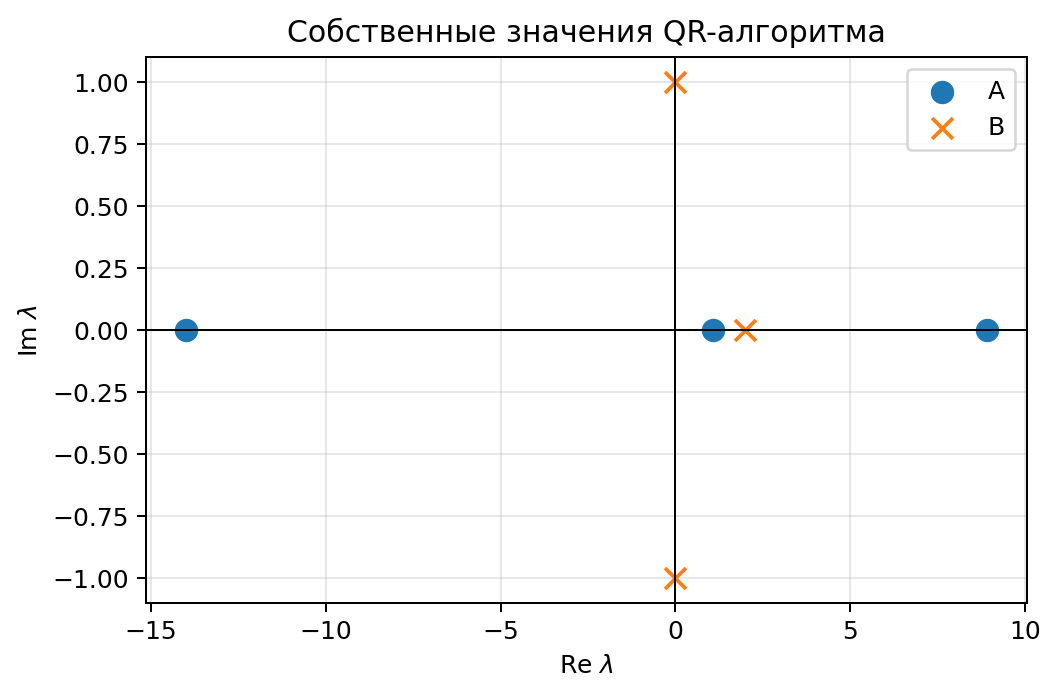
\includegraphics[width=0.86\textwidth]{lab1_5_eigenvalues.png}
    \caption{Собственные значения тестовых матриц на комплексной плоскости.}
\end{figure}

\section*{Выводы}
\addcontentsline{toc}{section}{Выводы}
QR-разложение на отражениях Хаусхолдера восстановило исходную матрицу с машинной точностью. QR-алгоритм успешно обработал как действительный спектр, так и комплексно-сопряженную пару, возникающую из двумерного блока.

\end{document}
